\documentclass{TDP003mall}

\usepackage{graphicx}
\usepackage{wrapfig}
\graphicspath{{images/}}

\newcommand{\version}{Version 1}
\author{Elliot Johansson, \url{elljo130@student.liu.se}\\
Nadim Lakrouz, \url{nadla777@student.liu.se}}
\title{System dokumentation}
\date{2022-10-11}
\rhead{Elliot Johansson\\
Nadim Lakrouz}



\begin{document}
\projectpage
\section{Revisionshistorik}
\begin{table}[!h]
\begin{tabularx}{\linewidth}{|l|X|l|}
\hline
Ver. & Revisionsbeskrivning & Datum \\\hline
1.0 & Skapa dokument samt lägga in bilder och text & 2022-10-11 \\\hline

\end{tabularx}
\end{table}

\section{index}
\begin{center}
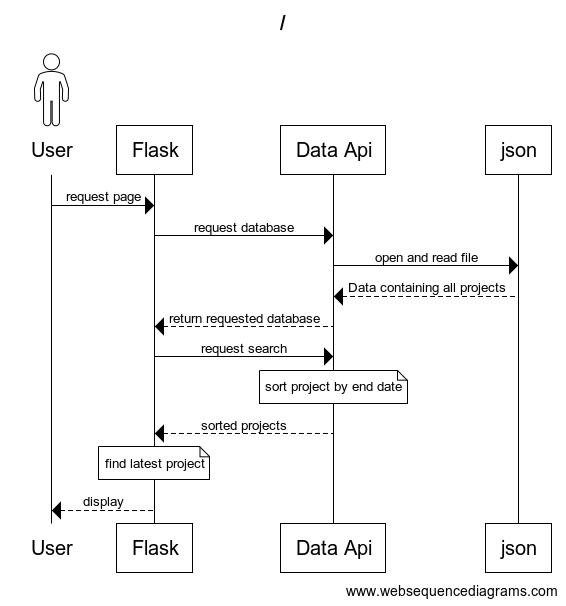
\includegraphics[scale=0.35]{index.png}
\end{center}
index() kör data.load() för att hämta databasen från json filen. Sen hämtar data.search() det senaste projektet och returnerar render-template() med index.html och det senaste projektet.\\\\

\section{list search}
\begin{center}
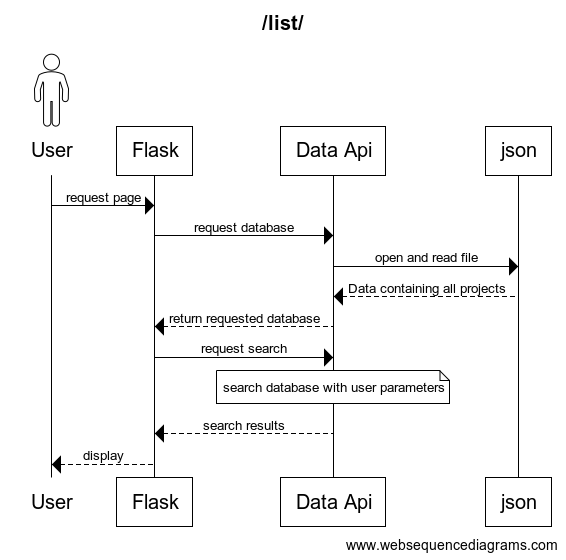
\includegraphics[scale=0.35]{list_search.png}
\end{center}
\begin{center}
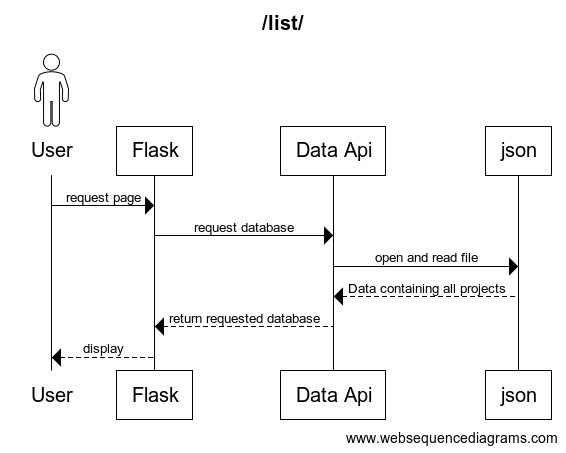
\includegraphics[scale=0.35]{list_no_search.png}
\end{center}
list() kör data.load() för att hämta databasen från json filen. Sedan kollar den om några argument returneras och om det gör det så körs data.search() med de argumenten och returnerar render-template() med list.html och renderar de projekt som kallas efter.\\\\



\section{project id}
\begin{center}
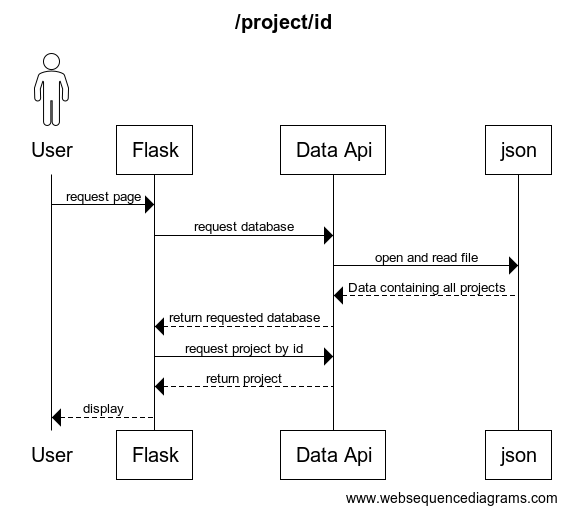
\includegraphics[scale=0.35]{project_id.png}
\end{center}
project(id) kör data.load() för att hämta databasen från json filen. Sedan kör den data.get-project() för att hämta projektet och sedan rendera det med render-template() i project.html. Om projektet inte finns körs error-404 istället.\\\\


\section{techniques}
\begin{center}
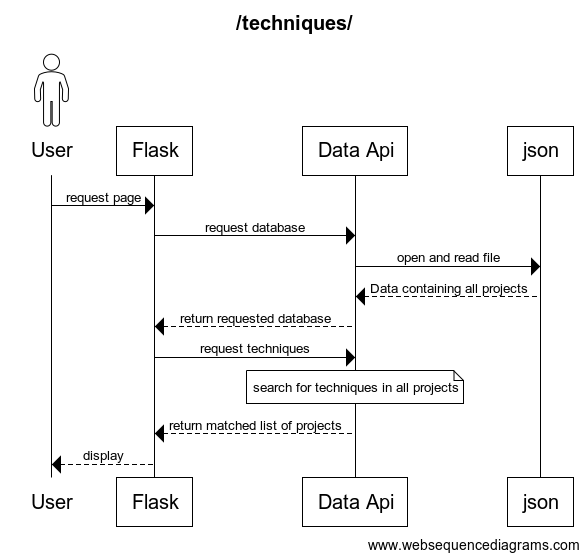
\includegraphics[scale=0.35]{techniques_.png}
\end{center}
techniques() kör data.load() för att hämta databasen från json filen. Sedan kör den data.get-technique-stats() och returnerar till slut alla projekt med techniques.html och render-template().
\section{errors}
När en sida som användaren försöker nå inte finns körs page-not-found() som returnerar error.html, error id och error meddelande. Om istället något blir fel med servern så körs server-error() som gör samma sak som page-not-found() fast den returnerar ett annat id och error meddelande.

\end{document}
